\subsubsection{Overview}
The Simplex Method is a popular algorithm to solve linear programs first
published by Dantzig \cite{dantzig_maximization_1951}. Conceptually, it is quite
intuitive, especially from a geometrical point of view. Before continuing in
more detail, an overview of the method is provided via the example from the
previous section. Take the linear program shown in Equation \ref{eqs:lp} and its
geometrical view shown in Figure \ref{fig:geometric}.

%%% 
\begin{subequations}\label{eqs:lp}
  \begin{align}
    %%
    \max \:\: & 
    f(x_1, x_2) = 3 x_1 + 2 x_2
    & \label{eqs:lp_obj} \\
    %%
    \text{s.t.} \:\: &
    -2 x_1 + x_2 \leq 1 \\
    %%
    &
    x_1 + x_2 \leq 5 
    & \label{eqs:lp_sup} \\
    %%
    &
    x_1 \leq 4
    &\label{eqs:lp_x1} \\
    %%
    &
    x_1, x_2 \geq 0
    &\label{eqs:lp_x2}
    %%
  \end{align}
\end{subequations}
%%% 

\begin{figure}[H]
  \begin{center}
    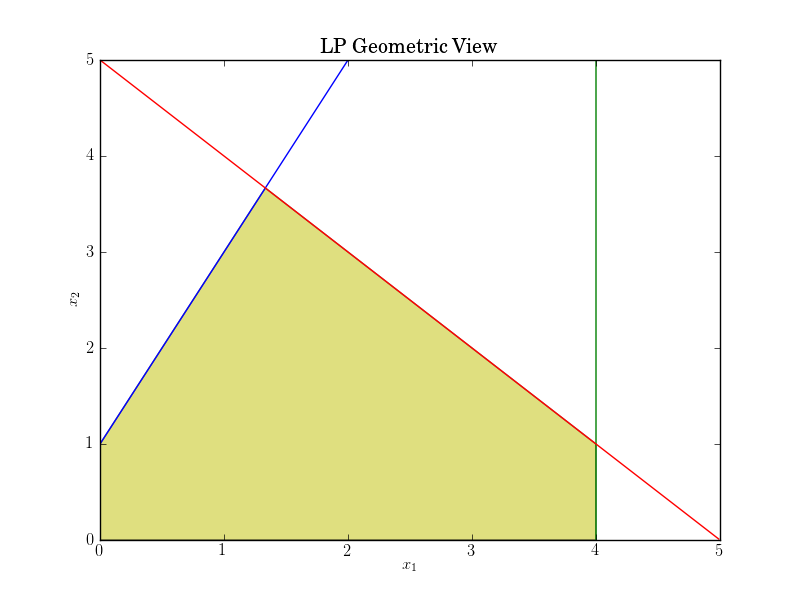
\includegraphics[height=7.5cm]{./chapters/litreview/plots/geometric.png}
  \caption{A Geometric View of the LP.}
  \label{fig:geometric}
  \end{center}
\end{figure}

Note that there are five vertices of the polygon (i.e., a polytope more
generally) formed by the full set of constraints:

\begin{enumerate}
  \item $(0, 0)$
  \item $(0, 1)$
  \item $(\frac{4}{3}, \frac{11}{3})$
  \item $(4, 1)$
  \item $(4, 0)$
\end{enumerate}

The Simplex Method begins at a vertex, for example $(0, 0)$, and evaluates the
objective function.

\begin{equation}
    f(0, 0) = 3 * 0 + 2 * 0 = 0 
\end{equation}

Neighbor vertices are then evaluated, in order to determine which provides the
larger value (in the case of maximizing objectives).

\begin{equation}
    f(0, 1) = 3 * 0 + 2 * 1 = 2 
\end{equation}

\begin{equation}
    f(4, 0) = 3 * 4 + 2 * 0 = 12 
\end{equation}

The vertex $(4, 0)$ provides a larger objective function value, so the algorithm
moves to this vertex and determines the next largest neighbor. In this simple
example, there is only one choice, and it is trivially larger.

\begin{equation}
    f(4, 1) = 3 * 4 + 2 * 1 = 14 
\end{equation}

Accordingly the algorithm moves a second time, analyzing the neighboring
vertices again.

\begin{equation}
    f(\frac{4}{3}, \frac{11}{3}) = 3 * \frac{4}{3} + 2 * \frac{11}{3} = \frac{34}{3} 
\end{equation}

At this last move, a terminating condition has been achieved: a vertex has been
found for which all of its neighbors provide a lower value for the objective
function, i.e.,

\begin{equation}
    14 \geq 12 \:\:\: \text{and} \:\:\: 14 \geq \frac{34}{3}.
\end{equation}

Thus, the optimal value for $(x_1, x_2)$ has been determined to be $(4, 1)$. It
is immediately obvious that the simplex algorithm in this state is a hill
climbing (or hill descending) algorithm. The chief reason why this is possible
(i.e., why one is guaranteed to find a globally optimum solution) is that the
objective function and constraints are \textit{convex} functions of the decision
variables. Convexification is requiried to find optimum solutions to both linear
and integer programs, and the concept is covered with slightly more detail
in \S \ref{sec:formulations}.

In general, the Simplex Method is efficient, i.e., for most cases solutiosn are
found in less than exponential time in the number of variables. There are
certain program structures for which solution times are exponential, however,
and it in such cases, more advanced \textit{Interior Point} techniques are
required. In general, Interior Point algorithms are often much faster than
Simplex Algorithms \cite{ferris_linear_2008}, but are beyond the scope of this
review. A more in-depth discussion of computational complexity is discussed
in \S \ref{sec:ip}.

\subsubsection{In-Depth Discussion}
To begin a more robust discussion of the Simplex Method, one must introduce the
notion of \textit{slack variables}. Slack variables are used to transform
inequality constraints into equality constraints, effectively taking the
``slack'' out of the system. Slack variables are always positive, thus one could
use a slack variable, $s$, to convert

\begin{equation}
  \sum_{i} a_i x_i \leq b
\end{equation}

to 

\begin{equation}
  \sum_{i} a_i x_i + s = b
\end{equation}

and

\begin{equation}
  \sum_{i} a_i x_i \geq b
\end{equation}

to 

\begin{equation}
  \sum_{i} a_i x_i - s = b.
\end{equation}

The addition of slack variables allows one to rewrite an LP given in the
standard form of Equation \ref{eqs:std-form} as the \textit{canonical form}.

%%% 
\begin{subequations}\label{eqs:can-form}
  \begin{align}
    %%
    \min_{x, s} \:\: & 
    z =  c^{\top} x + 0^{\top} s
    & \label{eqs:can-form_obj} \\
    %%
    \text{s.t.} \:\: &
    A x - b = s
    & \label{eqs:can-form_sup} \\
    %%
    &
    x, s \geq 0
    &\label{eqs:can-form_x}
    %%
  \end{align}
\end{subequations}
%%% 

Given that there are $N$ decision variables and $M$ constraints, the cardinality
of $x$ is $N$ and the cardinality of $s$ is $M$. Furthermore, in the literature,
the $x_i$ variables are termed \textit{nonbasic} variables whereas the $s_i$
variables are termed \textit{basic} variables.

For any LP in the canonical form, the Simplex Algorithm can be applied to it to
determine optimal values for its decision variables, or to determine that it is
unbounded or infeasible. The basic structure of the method is outlined below in
Algorithm \ref{alg:simplex}.

\begin{algorithm}[h!]
 \SetAlgoLined
 \KwData{Decision variables, an objective function, and a set of constraints.}
 \KwResult{Optimal values for the decision variables or a flag denoting 
   infeasibility or unboundedness.}
 Get initial vertex\;
 \If{no vertex is found}{
 feasible solution space is empty\;
 }
 \While{not unbounded and not empty and not done}{ 
    Select column, i, via pricing\;
    \If{no column is found}{
    optimal condition found\;
    done\;
    }
    Select row, j, via the ratio test\;
    \If{no row is found}{
    solution space is unbounded\;
    }
    Perform a Jordan exchange on element (i, j)\;
  }
  \caption{The Simplex Algorithm}\label{alg:simplex}
\end{algorithm}

There are four core operations associated with the Simplex Algorithm:
\begin{enumerate}
  \item finding an initial vertex
  \item column pricing
  \item row selection
  \item exchanging elements
\end{enumerate}

If finding an initial vertex is not trivial (e.g., if the origin is not a
candidate), then the operation to do so requires use of the Simplex Method on a
related LP where the origin is an available candidate. That process will be
described last.

The primary concept required to understand the Simplex Method's operations is
that of the \textit{basis}. The basis begins as the set of decision
variables. The algorithm progresses by moving slack variables into the basis,
and it does so efficiently by analyzing the most ``valuable'' variables to
target (i.e., which current basis variable affects the optimal value the most).

Column pricing and row selection are the operations that select the current
basis and nonbasis variables to target. The Jordan exchange process translates
the formulation into the new basis, exchanging basic and nonbasic
variables. This is perhaps more intuitive from a geometrical point of
view. Consider some starting vertex with many possible sides along which to
move. The process of column pricing and row selection \textit{chooses} the side
along which to move, and the Jordan exchange \textit{reorients} the
problem. Revisiting the example problem, remember the first step. The vertex
$(4, 0)$ was determined to be the best direction in which to move. After a
Jordan exchange, the resulting LP would look like Figure \ref{fig:rotated}.

\begin{figure}[H]
  \begin{center}
    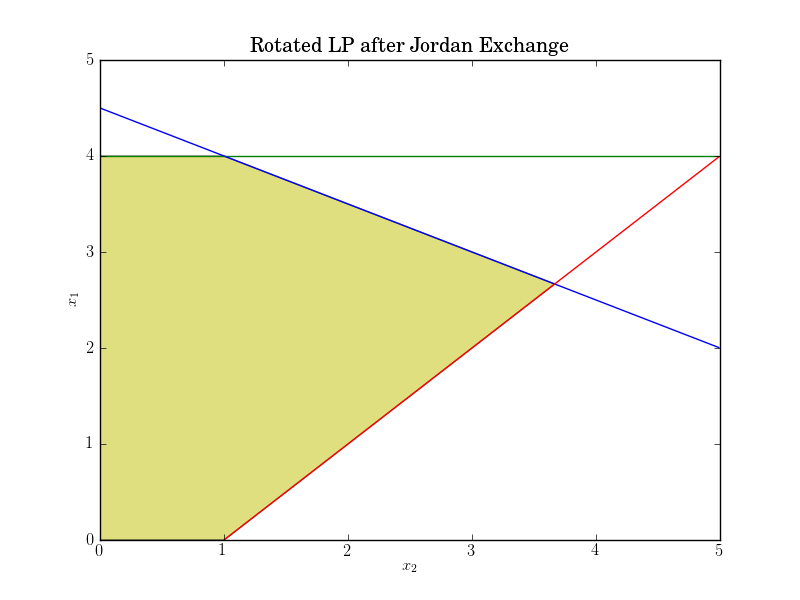
\includegraphics[height=7.5cm]{./chapters/litreview/plots/rotated.png}
  \caption{The Reoriented LP after the first Jordan Exchange.}
  \label{fig:rotated}
  \end{center}
\end{figure}

The column pricing operation selects the slack variable which will enter the
basis. The most naive implementation is to select the variable which will have
the largest effect on the objective function, i.e., which has the largest
magnitude \textit{reduced cost}. For instance, in Equation \ref{eqs:lp_obj},
$x_1$ has a reduced cost of 3, and $x_2$ has a reduced cost of 2 (note that both
costs are in the same positive direction as the objective, i.e.,
maximization). Accordingly, choosing $x_1$ as the nonbasic exchange variable is
a valid option. However, any algorithm may be used to make this selection, as
long as the reduced cost is positive.

Row selection, i.e., selecting the basic variable to enter the basis, is
performed via a ratio test. Given that a column $j$ has been selected, the
corresponding row is selected according to Equation \ref{eqs:ratio-max} in the
case of a maximization objective and Equation \ref{eqs:ratio-min} in the case of
a minimization objective.

\begin{equation}\label{eqs:ratio-max}
  \min \left\{ \frac{-b_i}{A_{i,j}} \:\: | \:\: A_{i,j} > 0 \right\}
\end{equation}

\begin{equation}\label{eqs:ratio-min}
  \min \left\{ \frac{-b_i}{A_{i,j}} \:\: | \:\: A_{i,j} < 0 \right\}
\end{equation}

The Jordan Exchange operation, which transforms a matrix $A \mapsto A'$
given a pivot $(\hat{\imath}, \hat{\jmath})$, is straightforward and is shown in
Equation \ref{eqs:jordan}.

%%% 
\begin{subequations}\label{eqs:jordan}
  \begin{align}
    %%
    a_{\hat{\imath},\hat{\jmath}}' = \frac{1}{a_{\hat{\imath},\hat{\jmath}}}
    &\:\: \text{for} \:
    i = \hat{\imath}, j = \hat{\jmath} \\
    %%
    a_{\hat{\imath},j}' = -\frac{a_{\hat{\imath},j}}{a_{\hat{\imath},\hat{\jmath}}}
    &\:\: \text{for} \:
    i = \hat{\imath}, j \neq \hat{\jmath} \\
    %%
    a_{i,\hat{\jmath}}' = \frac{a_{i,\hat{\jmath}}}{a_{\hat{\imath},\hat{\jmath}}}
    &\:\: \text{for} \:
    i \neq i, j = \hat{\jmath} \\
    %%
    a_{i,j}' = a_{i,j} - a_{i,\hat{\jmath}} a_{\hat{\imath},j}
    &\:\: \text{for} \:
    i \neq \hat{\imath}, j \neq \hat{\jmath}
    %%
  \end{align}
\end{subequations}
%%% 

Finally, one must determine a starting vertex. The original linear program is
modified as shown in \S 3.4 of \cite{ferris_linear_2008}. For each row, $i$, if
$b_i > 0$, then add an additional variable, $x_0$, to the constraint with
coefficient $a_{i,0} = 1$. An initial feasible point is then immediately
available for $x = 0 \:\: \forall \:\: i \neq 0$ and $x_0
= \max(\max(b),0)$. The Simplex Method is then applied, with $x_0$ being the
first variable to leave the basis. When $x_0$ returns to the basis, a suitable
starting vertex results from the removal of $x_0$.
